\subsection{Rohdaten von den Detektoren}
\begin{figure}
\centering
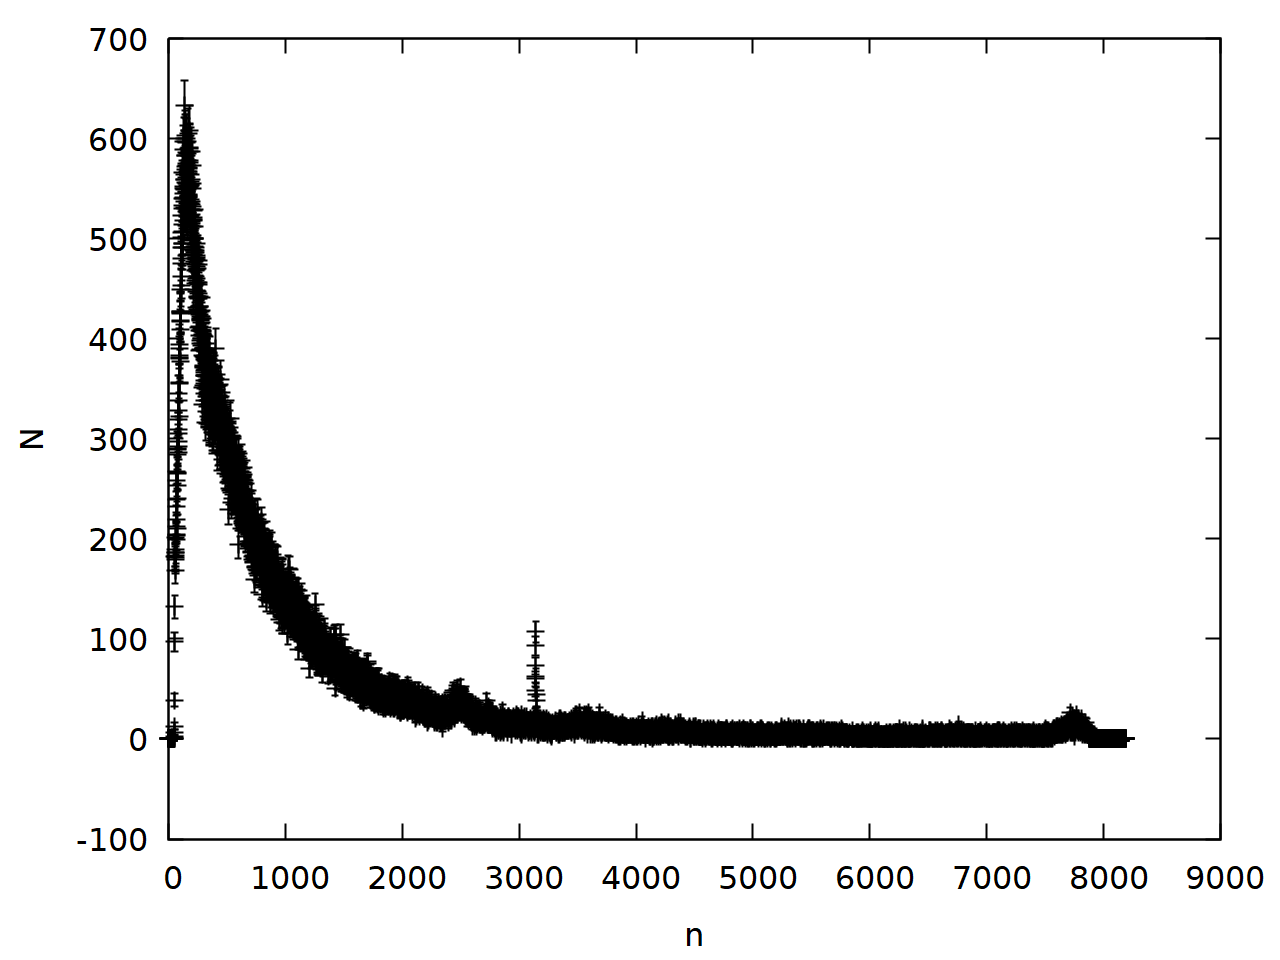
\includegraphics[width=0.7\linewidth]{data/si_unter.png}
\caption{Szintillator Untergrund}
\end{figure}

\begin{figure}
\centering
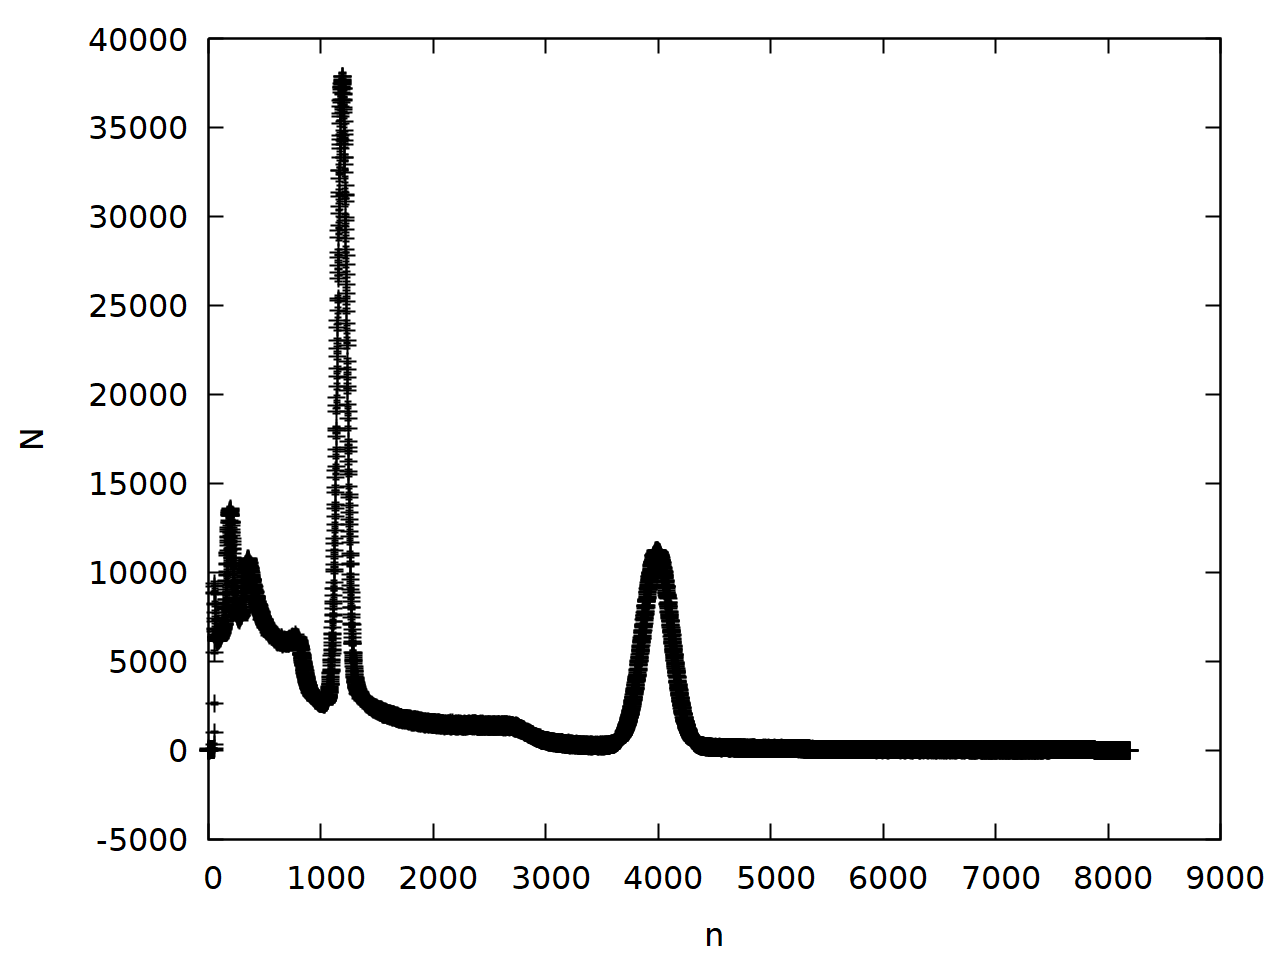
\includegraphics[width=0.7\linewidth]{data/si_cs_raw.png}
\caption{Szintillator Cs}
\end{figure}

\begin{figure}
\centering
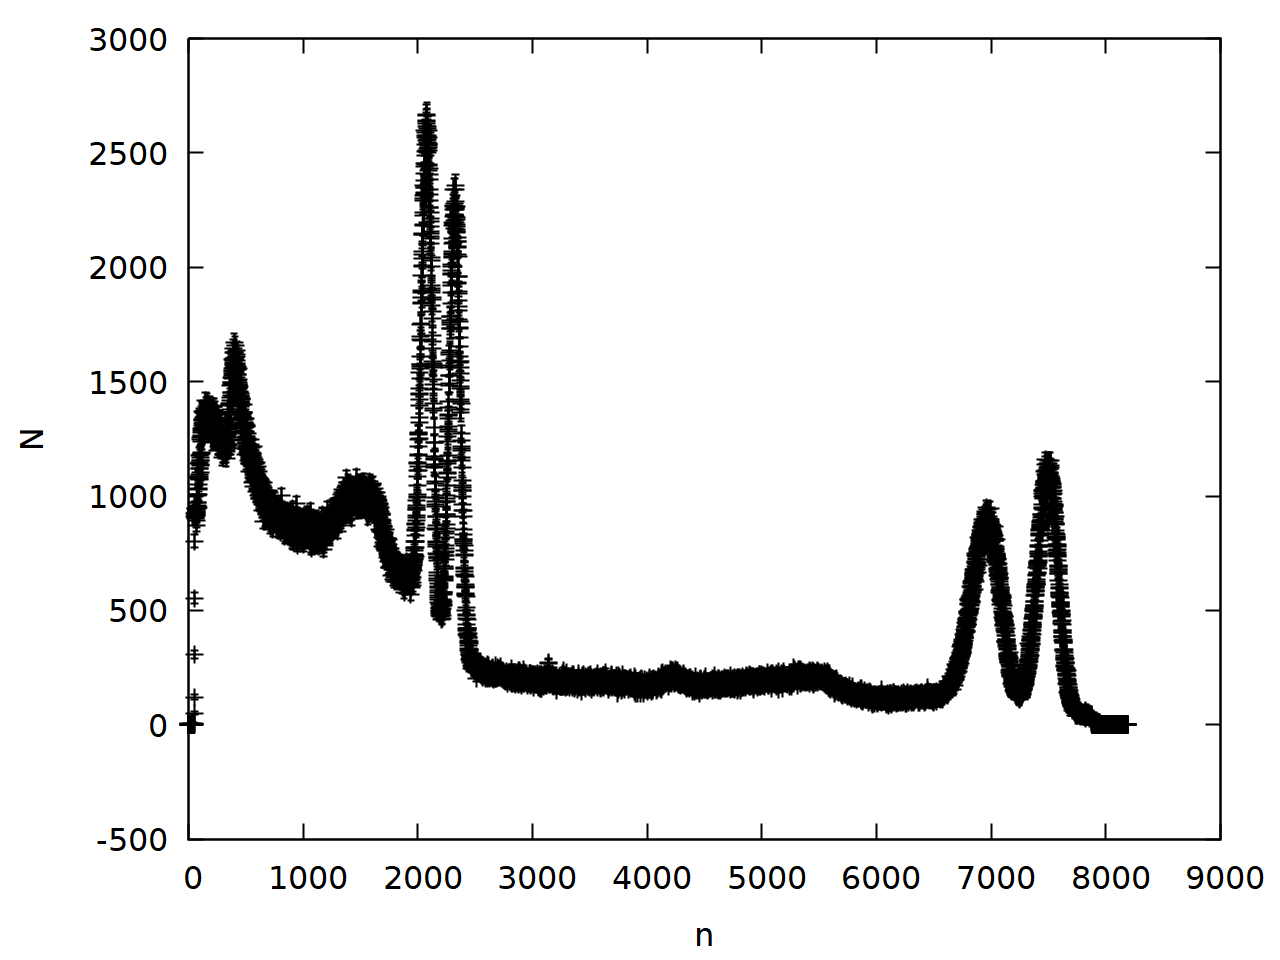
\includegraphics[width=0.7\linewidth]{data/si_co_raw.png}
\caption{Szintillator Co}
\end{figure}

\begin{figure}
\centering
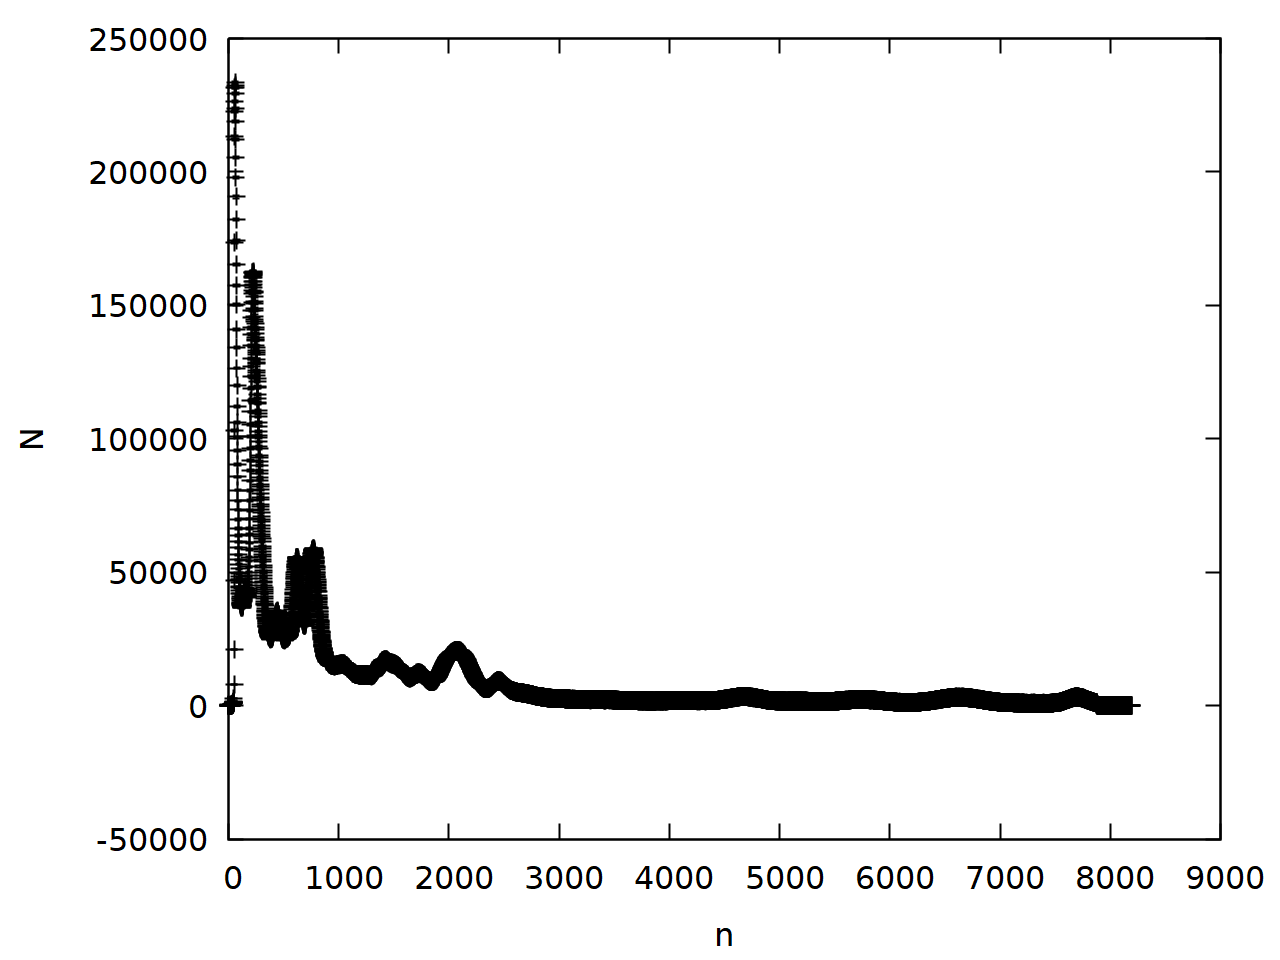
\includegraphics[width=0.7\linewidth]{data/si_eu_raw.png}
\caption{Szintillator Eu}
\end{figure}

\begin{figure}
\centering
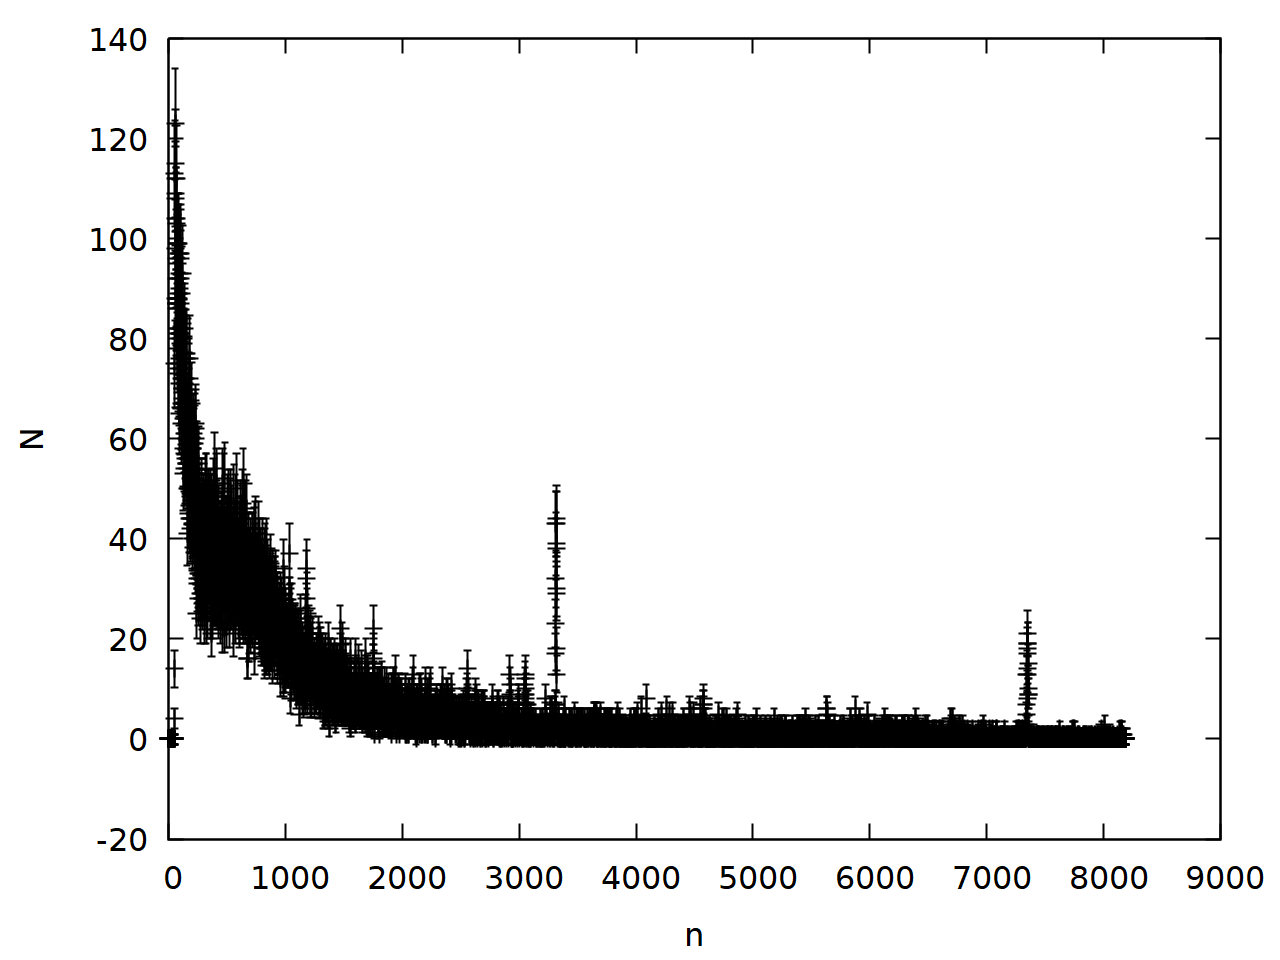
\includegraphics[width=0.7\linewidth]{data/ge_unter.png}
\caption{Germanium Untergrund}
\end{figure}

\begin{figure}
\centering
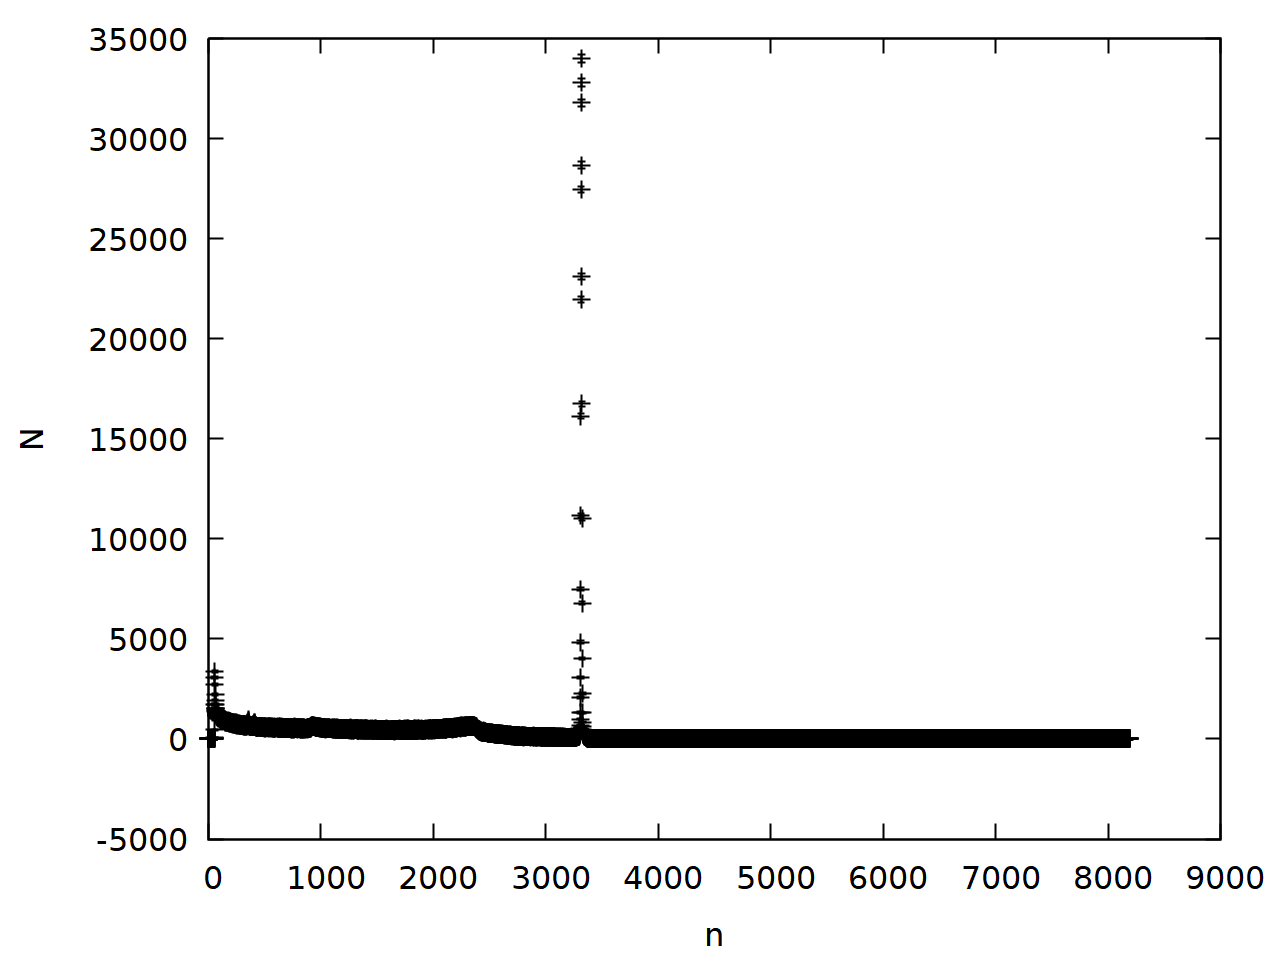
\includegraphics[width=0.7\linewidth]{data/ge_cs_raw.png}
\caption{Germanium Cs}
\end{figure}

\begin{figure}
\centering
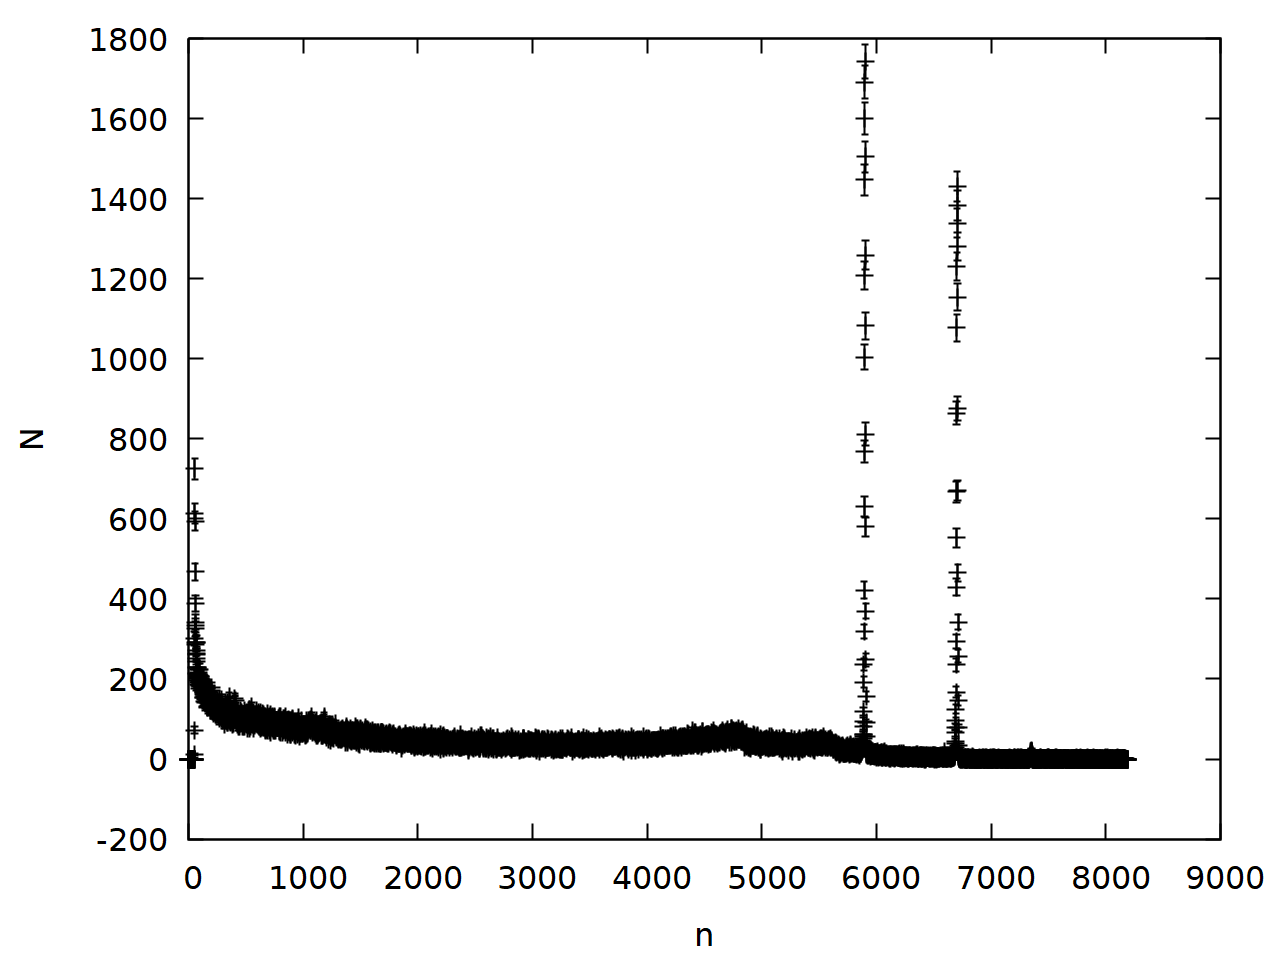
\includegraphics[width=0.7\linewidth]{data/ge_co_raw.png}
\caption{Germanium Co}
\end{figure}

\begin{figure}
\centering
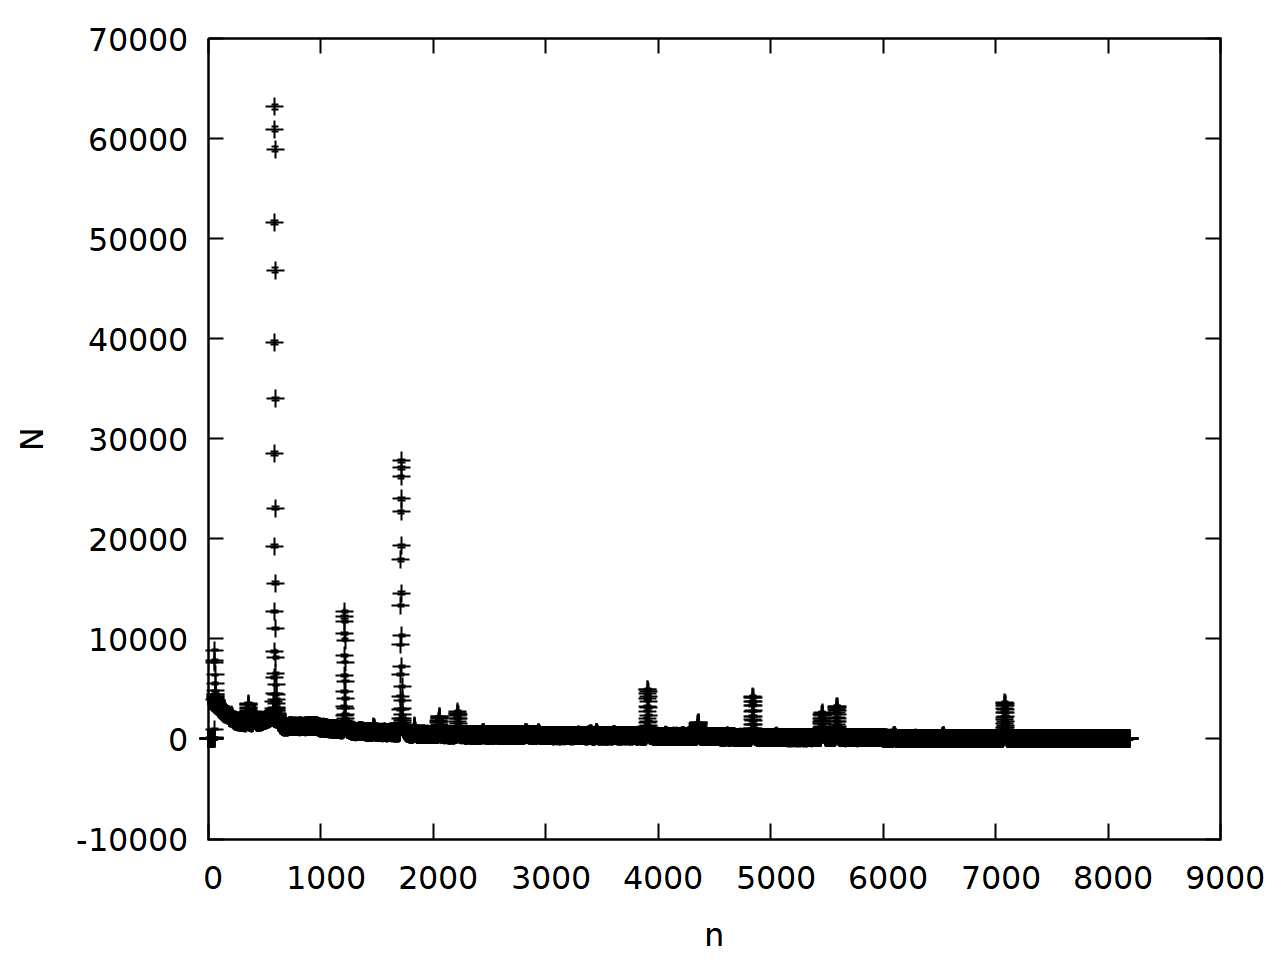
\includegraphics[width=0.7\linewidth]{data/ge_eu_raw.png}
\caption{Germanium Eu}
\end{figure}

\begin{figure}
\centering
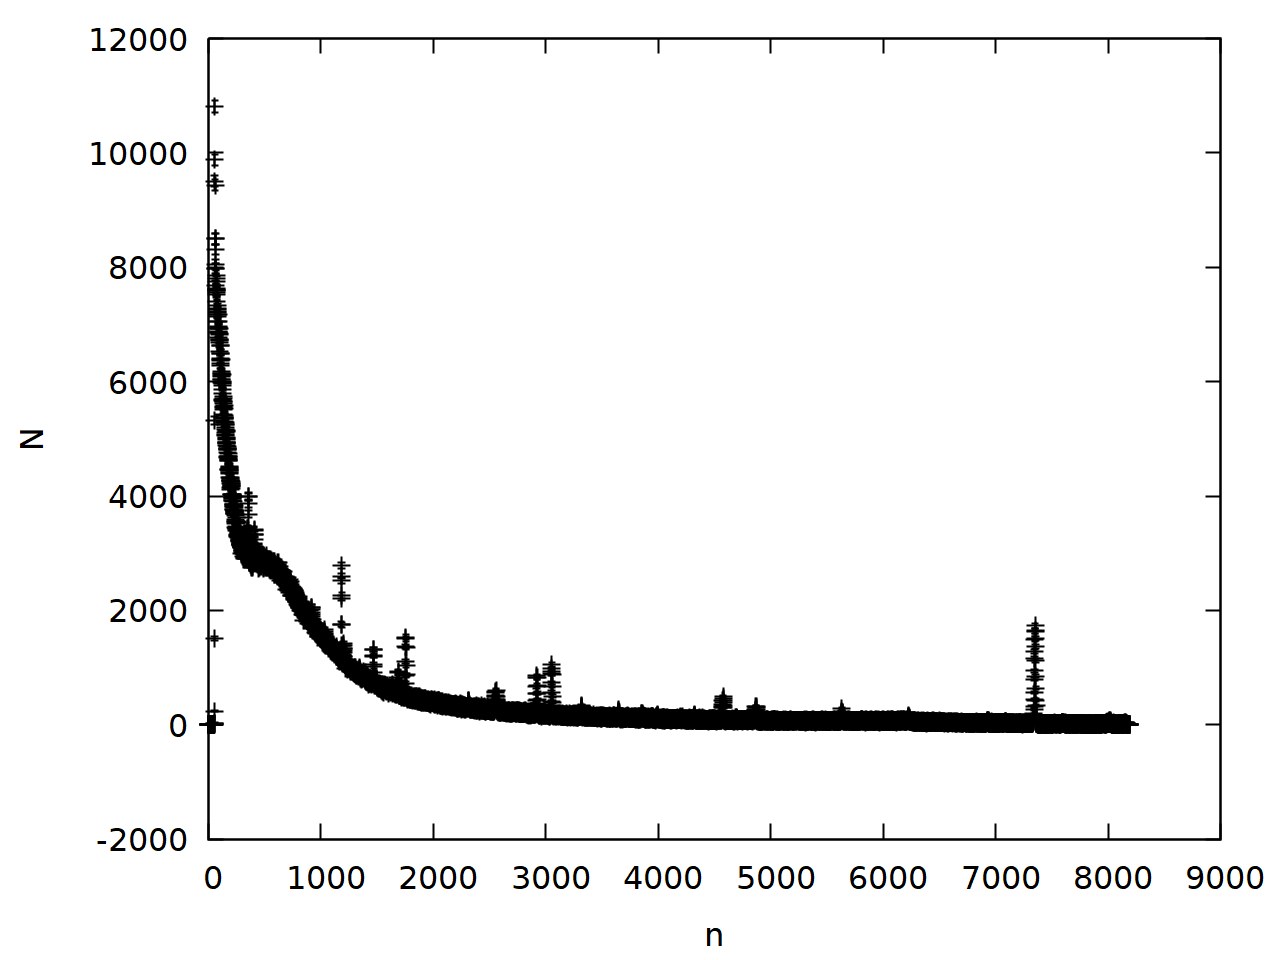
\includegraphics[width=0.7\linewidth]{data/erde_raw.png}
\caption{Bodenprobe}
\end{figure}

\begin{figure}
\centering
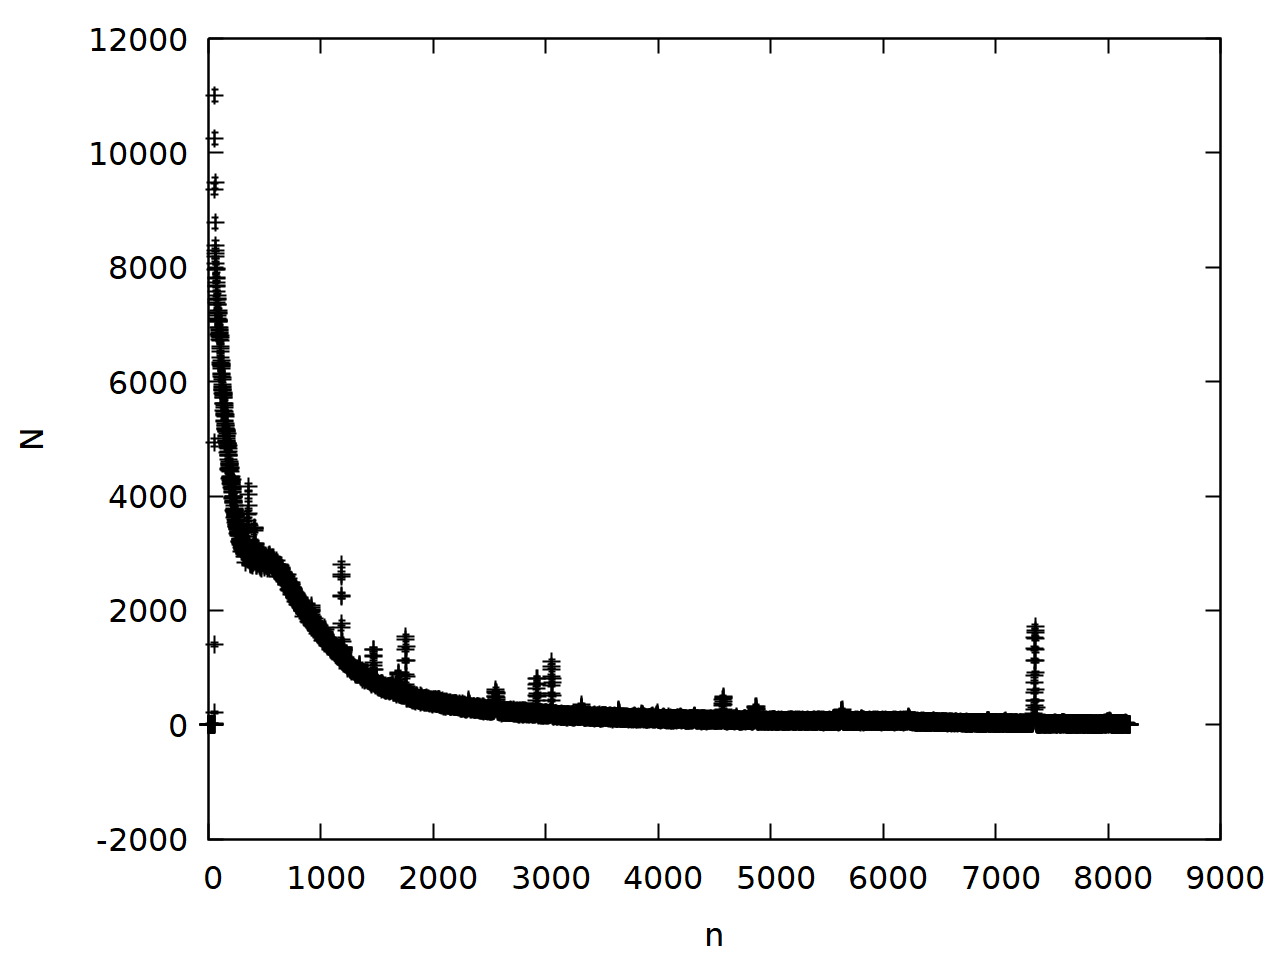
\includegraphics[width=0.7\linewidth]{data/untergrund.png}
\caption{Untergrundlangzeitmessung}
\end{figure}